\documentclass[bachelor, och, labwork]{shiza}

\usepackage[utf8]{inputenc}
\usepackage{graphicx}

\usepackage[sort,compress]{cite}
\usepackage{amsmath}
\usepackage{amssymb}
\usepackage{amsthm}
\usepackage{fancyvrb}
\usepackage{longtable}
\usepackage{array}
\usepackage[english,russian]{babel}
\usepackage{minted}

\usepackage{tempora}


% \usepackage[colorlinks=false]{hyperref}


\newcommand{\eqdef}{\stackrel {\rm def}{=}}


\begin{document}

\title{Схема Диффи -- Хеллмана}

\course{4}

\group{431}

\napravlenie{10.05.01 "--- Компьютерная безопасность}


\author{Никитина Арсения Владимировича}


\satitle{доцент}
\saname{А.\,В.\,Жаркова}


\date{2022}

\maketitle

% Включение нумерации рисунков, формул и таблиц по разделам
% (по умолчанию - нумерация сквозная)
% (допускается оба вида нумерации)
%\secNumbering


\tableofcontents





\section{Задание лабораторной работы}
Придумать схему разделения ключа аналогичную схеме Диффи -- Хеллмана между $n$
пользователями для $n \geqslant 3$.



\section{Теоретическая часть}

\subsection{Описание стандартного протокола Диффи -- Хеллмана}

Пусть известно большое конечное поле $F$ и порождающий элемент $g$ мультипликативной 
группы $F^*$. Двум абонентам А и В требуется выбрать секретным образом какое-нибудь
слу­чайное большое число  (секретный),  используя указанные данные в  качестве 
платформы.Сам выбор поля $F$ и порождающего элемента $g$ осуществляется по открытому
каналу, и поэтому данные $F$, $g$ являются открытыми.

Процесс разделения ключа между двумя пользователями можно разделить на следующие
составляющие:


\begin{enumerate}
    \item Установка;
    \item Генерация случайного числа и вычисление открытого ключа;
    \item Разделение ключа между пользователями.
\end{enumerate}

\begin{center}
    \textit{Установка}
\end{center}

Абоненты A и B договариваются о выборе поля $F$ и порождающего элемента $g$.
Для достижения криптостойкости наиболее приемлемым считается выбор такого поля
F, чтобы длина его была как минимум 2048 бит, а также чтобы оно было простым, 
причем $(F - 1 )/ 2$ также должно быть простым числом.

\begin{center}
    \textit{Генерация случайного числа и вычисление открытого ключа}
\end{center}

Абонент A выбирает случайным образом натуральное число $x$ и вычисляет $y \equiv g^x ~(mod ~F)$
и передает $y$ абоненту B.

Абонент B выбирает случайным образом натуральное число $z$ и вычисляет $u \equiv g^z ~(mod ~F)$
и передает $u$ абоненту A.

\begin{center}
    \textit{Разделение ключа между пользователями}
\end{center}

Абонент A, зная $x$ и $u$ вычисляет элемент $u^x \equiv g^{zx} ~(mod~F)$.

Абонент A, зная $z$ и $y$ вычисляет элемент $y^z \equiv g^{xz} ~(mod~F)$.

Таким образом, абоненты получили одно и то же число, причем никто кроме их самих
этим ключом не владеет.

\subsection{Описание алгоритма для большего количества пользователей}

Пусть ключ требуется разделить между n пользователями: $n \geqslant 3, ~ A_1,A_2, ...,A_n$.

Выполним аналогичные операции для большего количества пользователей. Для этого
заметим, что если требуется разделить ключ между одним пользователем и всеми
остальными, то он должен быть последним пользователем, к которому попадет исходное
число после всех возведений его в степень.

\begin{center}
    \textit{Установка}
\end{center}
Абоненты $A_1,..,A_n$ договариваются о выборе поля $F$ и порождающего элемента $g$.

\begin{center}
    \textit{Генерация случайного числа и вычисление открытого ключа}
\end{center}

Пусть каждый абонент $A_1,...,A_n$ выбрал свое случайное число $s_{A_i}$ и сгенерировал
свой открытый ключ $O_i \equiv g ^ {s_{A_i}} ~(mod ~ F)$ ($i = \overline{1, n} $).

Заметим, что если абонент $A_i$ передал свой открытый ключ другому абоненту, то
на данном шаге получить свой разделенный закрытый ключ он никак не сможет, поэтому
генерация открытого ключа абонентом и передача его по открытому каналу связи будет
свидетельствовать о том, что началась новая цепочка передач ключа.

\begin{center}
    \textit{Разделение ключа между пользователями}
\end{center}

Воспользуемся следующим свойством коммутативности показателей при последовательном
возведении в степень:
\begin{center}
    $(g^b ~mod ~ p)^ a ~ mod ~ p \equiv (g ^ a ~ mod ~ p) ^ b ~ mod ~ p \equiv g ^ {ab} ~ mod ~ p$
\end{center}

Таким образом, можно рассмотреть последовательное возведение в степень не только
для двух показателей, но и для большего их количества.

Имеем n пользователей: $A_1, A_2, ... , A_n$. 

Все вычисления производятся в по модулю $p$:

\begin{enumerate}
    \item Пользователь $A_1$ вычисляет $g^{s_{A_1}}$ и передет результат пользователю $A_2$
    \item Пользователь $A_2$ вычисляет $g^{s_{A_1} \cdot s_{A_2}}$ и передает результат пользователю $A_3$
    \item $\cdots$
    \item Пользователь $A_n$ вычисляет $g^{(s_{A_1} \cdot s_{A_2} ... \cdot s_{A_{n-1}}) \cdot s_{A_n}}$ и получает общий секретный ключ.
    \item Затем пользователь $A_2$ вычисляет $g^{s_{A_2}}$ и передет результат пользователю $A_3$
    \item Пользователь $A_3$ вычисляет $g^{s_{A_2} \cdot s_{A_3}}$ и передает результат пользователю $A_4$
    \item $\cdots$
    \item Пользователь $A_n$ вычисляет $g^{s_{A_2} \cdot s_{A_3} ... \cdot s_{A_n}}$ и передет результат пользователю $A_1$.
    \item Пользователь $A_1$ вычисляет $g^{(s_{A_2} \cdot s_{A_3} ... \cdot s_{A_{n}}) \cdot s_{A_n}}$ и получает общий секретный ключ. 
    \item Таким образом, общий секретный ключ будет получен для всех пользователей.
\end{enumerate}

Для пользователя с номером $k: 2 \leq k < n$ секретный ключ будет вычисляться по
формуле:
\begin{center} $(((((g ^ {s_{A_{k+1}}} ~ mod ~ p) ^ {s_{A_{k+2}}} ~ mod ~ p ...) ^ 
    {s_{A_n}} ~ mod ~ p) ^ {s_{A_1}} ~ mod ~ p...)^ {s_{A_{k-1}}} ~ mod ~ p) ^ 
    {s_{A_k}} ~ mod ~ p \equiv (g^{s_{A_1}\cdot ... \cdot s_{A_{k-1}} \cdot 
    s_{A_{k+1}} \cdot ... \cdot s_{A_{n}}} ~mod ~p) ^ {s_{A_k}} ~mod ~ p
    \equiv g^{s_{A_{1}}\cdot ... \cdot s_{A_{k-1}} \cdot s_{A_{k+1}} \cdot ... \cdot s_{A_{n}} \cdot {s_{A_k}}} ~mod ~ p$.
\end{center}

Для пользователя с номером $k=1$ секретный ключ будет вычисляться по
формуле:
\begin{center} 
    $(((g ^ {s_{A_2}} ~ mod ~ p)^ {s_{A_3}} ~mod ~p...)^ {s_{A_n}} ~ mod ~ p) ^ 
    {s_{A_1}} ~ mod ~ p  \equiv (g^{s_{A_2}\cdot ... \cdot s_{A_{n}}} ~mod ~ p) ^ 
    {s_{A_k}} ~mod ~ p \equiv g^{s_{A_2}\cdot ... \cdot s_{A_{n}} \cdot {s_{A_k}}} ~mod ~ p$.

\end{center}
Для пользователя с номером $k=n$ секретный ключ будет вычисляться по
формуле:
\begin{center} 
    $(((g ^ {s_{A_1}} ~ mod ~ p)^ {s_{A_2}} ~mod ~p...)^ {s_{A_{n-1}}} ~ mod ~ p) ^
     {s_{A_n}} ~ mod ~ p \equiv (g^{s_{A_1}\cdot ... \cdot s_{A_{n - 1}}} ~mod ~ p) ^ 
     {s_{A_k}} ~mod ~ p \equiv g^{s_{A_1}\cdot ... \cdot s_{A_{n-1}} \cdot {s_{A_k}}} ~mod ~ p$.
\end{center}

\section{Практическая часть}
\subsection{Пример работы алгоритма}
\begin{figure}[H]
    \centering
    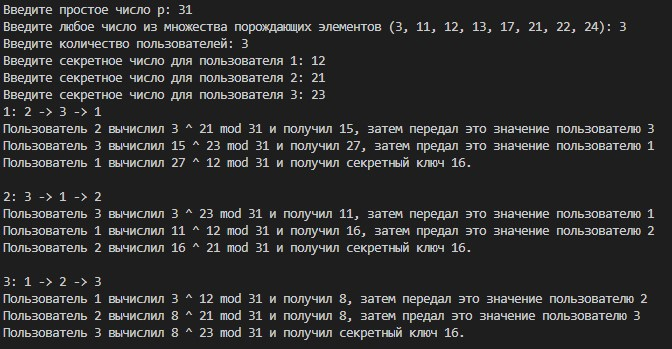
\includegraphics[width=0.8\textwidth]{pic.jpg}
    \caption{}
\end{figure}

\setminted[python]{linenos,breaklines=true, fontsize=\small, style=bw}
    \subsection{Код программы, реализующей рассмотренный алгоритм}
        \inputminted{python}{lab6.py}

\end{document}